% !TEX encoding = UTF-8
% !TEX TS-program = pdflatex
% !TEX root = ../arsclassica.tex
% !TEX spellcheck = it-IT

%************************************************
\chapter{Guide all'uso}
\label{cap:guide}
%************************************************

\section{Utilizzo del package CTBN}\label{sec:package-howto}
\omissis{}

\subsection{Caricamento del dataset}

\subsection{Calcolo delle sufficient statistics}

\subsection{Calcolo dei parametri}

\subsection{Calcolo delle CIM}

\subsection{Apprendimento}

\subsection{Classificazione}

\subsection{Apprendimento strutturale}

\subsection{Cross-validation}

\section{Creazione di dataset}\label{sec:create-dataset-howto}
In questa sezione si illustra il processo di generazione di un dataset per le \acs{CTBN} a partire da un modello di traffico \acs{TSIS}, utilizzando l'\acl{RTE} sviluppata in questo lavoro di tesi, \acsfont{Sensors} \acs{DLL}.

\subsection{Sensors DLL}
Al fine di generare un dataset per le \acs{CTBN} che rappresenti l'\keyword{onda quadra} dei sensori a spira magnetica posti su una rete stradale \acs{TSIS} è necessario installare \acsfont{Sensors} \acs{DLL} in \acs{TShell}. Il processo di installazione, come già ampiamente specificato, consiste nel collegamento delle funzioni della succitata \acs{RTE} ai punti di chiamata predefiniti del modulo \acs{CORSIM}. L'intero processo di installazione, propedeutico alla generazione dei dataset, è stato illustrato nella \autoref{subsec:rte-corsim-linking} \vpageref{subsec:rte-corsim-linking}.

Si mostra il processo di generazione del \ds{2} (\vref{sec:dataset-2}).

Come primo passo è chiaramente necessario aprire \acs{TSIS} \acsfont{Next}, cioè l'ultima versione di \acs{TShell} (versione $6.3$), e caricare il modello di traffico per i giorni lavorativi relativo a \emph{Viale Cesare Battisti}. Di seguito si elencano quindi i passi necessari alla generazione del \ds{2}:
\begin{itemize}
	\item dal \emph{menù} delle \emph{opzioni} si selezioni la voce \emph{proprietà d'esecuzione} e successivamente la scheda \emph{proprietà d'esecuzione multipla}
	\item si selezioni il file \acs{RNS} fornito in allegato a questo lavoro di tesi (e riportato in \vref{lst:model2-week-rns})\par
	\begin{minipage}{\linewidth}
		\centering
		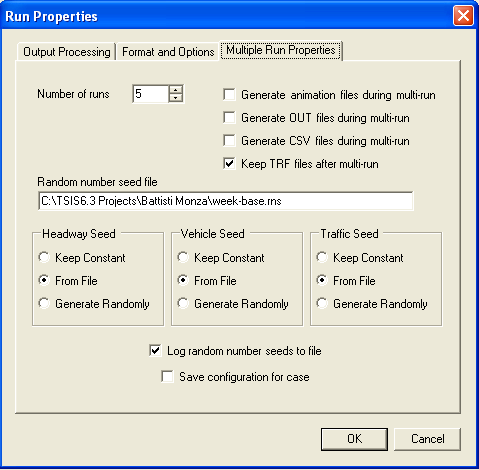
\includegraphics[width=1\linewidth]{multi-run-properties-tsis-next}\captionof{figure}[Esecuzione multipla guidata da file \acs{RNS}]{Selezione del file \acs{RNS} per l'impostazione dell'esecuzione multipla.}\label{fig:multi-run-properties-tsis-next}
	\end{minipage}
	\item \omissis{}

\end{itemize}

\subsection{Applicativi di supporto}
\omissis{}


